\chapter{Dynamic Query Expansion}
\markright{Aravindan Mahendiran \hfill Chapter 2. Dynamic Query Expansion\hfill}
\section{Query Expansion}
In most document corpora, a single concept can be referred using multiple terms.
In information retrieval (IR) this is called \emph{synonymy} and has a huge impact on the recall of documents pertaining to the concept.
Researchers address this problem by creating as exhaustive a query as possible. 
But when exploring the Twitter corpora it becomes almost impossible to hand craft such a expansive query as the meme and hashTag adaptations are not known a priori. 
\newline
To address this issue IR experts use \emph{query expansion} or re-inforcement learning.
These are iterative algorithms that are initialized with a small set of query terms. 
When the documents matching the query terms are returned, after basic NLP processing such as tokenization, stop-word removal and stemming a richer vocabulary is obtained by ranking the terms in these documents by their frequency counts.
The top n words from this list is then used to query the documents again. 
The iterations are stopped when no new terms are added to the vocbulary. 
We implement such an algorithm using Probabilistic Soft Logic to build our vocabulary for a given election.
\section{Probabilistic Soft Logic}
Probabilistic Soft Logic ~\cite{kimmig2012short} is a framework for collective probabilistic reasoning on relational domains.
PSL models have been developed in various domains, including collective classification ~\cite{broecheler2010computing}, ontology alignment ~\cite{brocheler2012probabilistic}, personalized medicine ~\cite{bach2010decision}, opinion diffusion ~\cite{bach2012scaling} , trust in social networks ~\cite{huang2012probabilistic}, and graph summarization ~\cite{memory2012graph}.
PSL represents the domain of interest as logical atoms.
It uses first order logic rules to capture the dependency structure of the domain, based on which it builds a joint probabilistic model over all atoms.
Instead of hard truth values of $0$ (false) and $1$ (true), PSL uses soft truth values relaxing the truth vlaues to the interval $[0,1]$.
The logical connectives are adapted accordingly.
This makes it easy to incorporate similarity or distance functions.
\newline
User defined \emph{predicates} are used to encode the relationships and attributes and \emph{rules} capture the  dependencies and constraints.
Each rule's antecedant is a conjunction of atoms and its consequent is a disjunction. 
The rules can also labled with non negative weights which are used during the inference process. 
The set of predicates and weighted rules thus make up a PSL program where known truth values of ground atoms derived from observed data and unknown truth values for the remaining atoms are learnt using the PSL inference.
\newline
Given a set of atoms 
$\ell = \{\ell_1,\ldots,\ell_n\}$,
an interpretation defined as 
$I : \ell \rightarrow [0,1]^n$
is a mapping from atoms to soft truth values.
PSL defines a probability distribution over all such interpretaions such that those that satisfy more ground rules are more probable.
\emph{Lukasiewicz t-norm} and its corresponding co-norm are used for defining relaxations of the logical AND and OR respectively to determine the degree to which a ground rule is satisfied.
Given an interpretation $\mathit{I}$, PSL defines the formulas for the relaxation of the logical conjunction ($\wedge$), disjunction ($\vee$), and negation ($\neg$) as follows:

\begin{align*}
\ell_1 \softand \ell_2 &= \max\{0, I(\ell_1) + I(\ell_2) - 1\},\\
\ell_1 \softor \ell_2 &= \min\{I(\ell_1) + I(\ell_2), 1\},\\
\softneg l_1 &= 1 - I(\ell_1),
\end{align*}  

The interpretation $\mathit{I}$ determines whether the rules is satisfied, if not, the \emph{distance to satisfaction}.
A rule $\mathit{r} \equiv \mathit{r_{body}} \rightarrow \mathit{r_{head}} $  is satisfied if and only if the truth value of head is atleast that of the body. The rule's distance to satisfaction measures the degree to which this condition is violated.
 \newline
\begin{center} 
 $\mathit{d_r}(\mathit{I}) =$ max\{0,$\mathit{I(r_{body}} - \mathit{I(r_{head}}$\}
 \end{center}

PSL then induces a probability distribution over possible interpretations $\mathit{I}$ over the given set of ground atoms $\mathit{l} $ in the domain. 
If $\mathit{R}$ is the set of all ground rules that are instances of a rule from the system and uses only the atoms in  $\mathit{I}$ then,
the probability density function $\mathit{f}$ over $\mathit{I}$ is defined as
\begin{equation}
\label{eq:contimn1}
    f (I) = \frac{1}{Z} \text{exp}[-\sum_{r\in R} \lambda_r (d_r(I))^p]
\end{equation}
\begin{equation}
\label{eq:contimn2}
	Z = \int_{I} \text{exp} [ -\sum_{r\in R} \lambda_r (d_r(I))^p ]
\end{equation}
where~$\lambda_r$ is the weight of the rule~$r$, $Z$ is the continuous version of the normalization constant used in discrete Markov random fields, and ~$p \in \{1, 2\}$ provides a choice between two different loss functions, linear and quadratic.
The values of the atoms can be further restricted by providing linear equality and inequality constraints allowing one to encode functional constraints from the domain. 
PSL provides for two kinds of inferences (a)most probable explanation and (b)calculation of the marginal distributions. 
In the MPE inference given a partial interpretation with grounded atoms based on observed evidence, the PSL program infers the truth values for the unobserved atoms satisfying the most likely interpretation. 
In the second setting, given ground truth data for all atoms we can learn the weights for the rules in our PSL program.
\section{Query Expansion using PSL}
In ~\cite{huang2012social}, we used PSL to model user affiliations within groups. 
Specifically we built a PSL program for a  social network where we have a set of users, their posts, messages to other users and the various groups we want to model. 
The rules we defined captured the dynamics of group affiliations through the various interactions.
Through the MPE inference we classified users into different groups based on their hashtag usage and their interactions with other users.
\newline
In this paper we extend our earlier work to achieve what we call dynamic query expansion through PSL. 
Similar to the query expansion methodology described earlier we start with an initial set of key words which we believe are indicative of the affinity of a particular user to a candidate contesting in the election.
Now instead of a single inference, we iteratively perform the inference over successive time windows such that the inference from window $w_t$ is used as a prior to window $w_{t+1}$ and the inference from that is used for window $w_{t+2}$ and so on.
In order to capture the temporal connectivity between the iterations, in addition to the adaptation of rules from ~\cite{huang2012social} we define additional rules and predicates as follows:
\begin{align*}
Was\_Member(A,G) \Rightarrow Is\_Memeber(A,G)
\end{align*}
\begin{align*}
Belonged(W,G) \Rightarrow Belongs(W,G)
\end{align*}
Here the predicates $Was\_Member$ and $Belonged$ are inferences from the previous time window and are loaded in as  prior to the current iteration.
These rules are weighted slightly lower than the recursive rules below so that the system overcomes the bias it had learnt in light of new more convincing evidence.
This way hashtags that are more indicative of a user's affiliation move up in the ranking for every successive iteration and the hashtags that aren't move down.
A similar phenomenon occurs with the user-candidate affiliations too.
Below we outline the recursive PSL rules that grows the hashtag preferences and the user affiliations. 
\begin{align*}
\begin{split}
Tweeted(A,T) 
	\softand Contains(T,W)
	\softand Belongs(W,G) \\ 
	\softand Positive(T)
	\Rightarrow Is\_Member(A,G)
\end{split}
\end{align*}

\begin{align*}
\begin{split}
Tweeted(A,T)
	 \softand Contains(T,W)
	\softand Belongs(W,G)\\
	 \softand Negative(T)
	\Rightarrow \sim Is\_Member(A,G)
\end{split}
\end{align*}

\begin{align*}
\begin{split}
Is\_Member(A,G)
	 \softand Tweeted(A,T)
	\softand Contains(T,W)\\
	 \softand Positive(T) 
	\Rightarrow Belongs(W,G)
\end{split}
\end{align*}

\begin{align*}
\begin{split}
Is\_Member(A,G) 
	\softand Tweeted(A,T)
	\softand Contains(T,W)\\
	\softand Negative(T)
	\Rightarrow \sim Belongs(W,G)
\end{split}
\end{align*}

\begin{align*}
\begin{split}
Contains(T,W1)
 \softand Contains(T,W2)
  \softand Belonged(W1,G)\\ 
  \softand Positive(T)
	\Rightarrow Belongs(W2,G)
\end{split}
\end{align*}

\begin{align*}
\begin{split}
Contains(T,W1) 
	\softand Contains(T,W2)
	\softand Belonged(W1,G)\\ 
	\softand Negative(T)
	\Rightarrow \sim Belongs(W2,G)
\end{split}
\end{align*}

Here $Positive$ and $Negative$ are predicates whose truth values are calculated from the sentiment of the tweet such that the highly positive tweets get a truth value closer to $1.0$ for the predicate $Positive$. 
Since PSL works under the close world assumption, we do not need to specify the groundings that are false.
For tweets that do not have a positive or negative orientation we assign a truth value of $0.5$ for both the $Positive$ and $Negative$ predicates.
The last two rules are added to encode the belief that hashtags occuring together are expected to be about the same group.
%\paragraph{}
For every iteration, we collect tweets from the country of interest that was created within the time window and filter the tweets that contain any hashtag from the previous inference  or that has been authored by or directed at a user whose affiliation is already known from the previous iterations.
We believe this helps us start with as little bias as possible and improve our learning with every time window.
From various experiments conducted we noticed that we get best results for a window size of 3 days. 
We begin this iterative approach by tracking tweets from 1 month prior to the election and thereby hoping to capture the changing trends in the use of hashTags.
At the end of each iteration we are get each hashtag's probability of belonging to a particular candidate's vocabulary. 
We normalize the each hashtag's weight over all previous time windows so that we identify hashtags that have remained indicative of a user's affiliation for the longest period of time without dropping in importance. 
We then use the top hashtags ranked according to their normalized weights  for the next iteration.
This normalization reduces the influx of hashtags that are in vogue only for a specific time window and are not as indicative of user affiliation for the entire time period. 
\subsection{Performance}
% word growth figure
\begin{figure*}[Ht]
	\centering
	%\captionsetup{font=scriptsize}
	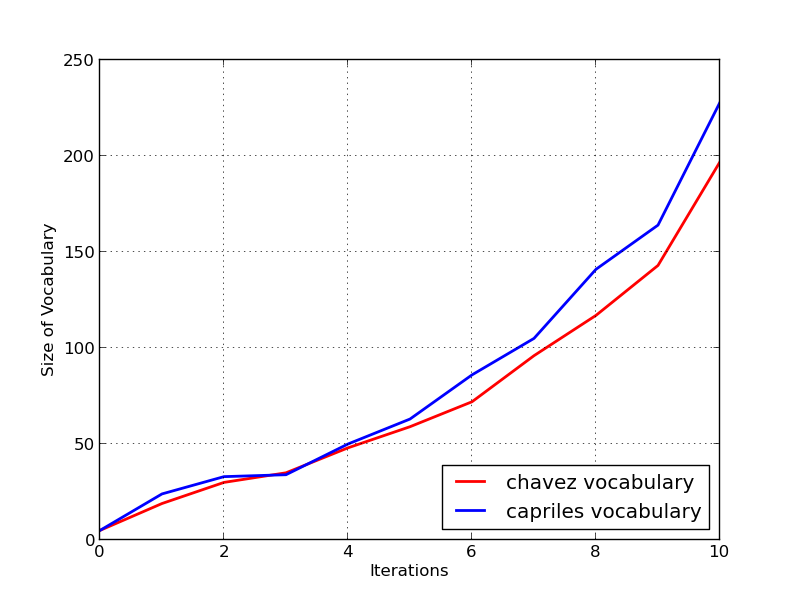
\includegraphics[width=0.7\textwidth, height=0.3\textheight]{/Users/aravindan/Dropbox/git/ms_thesis/documentation/my_thesis/support_files/WordGrowth.png}
	\vspace{-1em}
	\caption{Word growth over time}
	\label{fig:wordgrowth}
	\vspace{-1em}
\end{figure*}	
Figure\ref{fig:wordgrowth} shows the growth of the vocabulary with every iteration for the Venezuelan presidential election in 2012.
% word cloud figure
\begin{figure*}[ht]
	\centering
	%\captionsetup{font=scriptsize}
	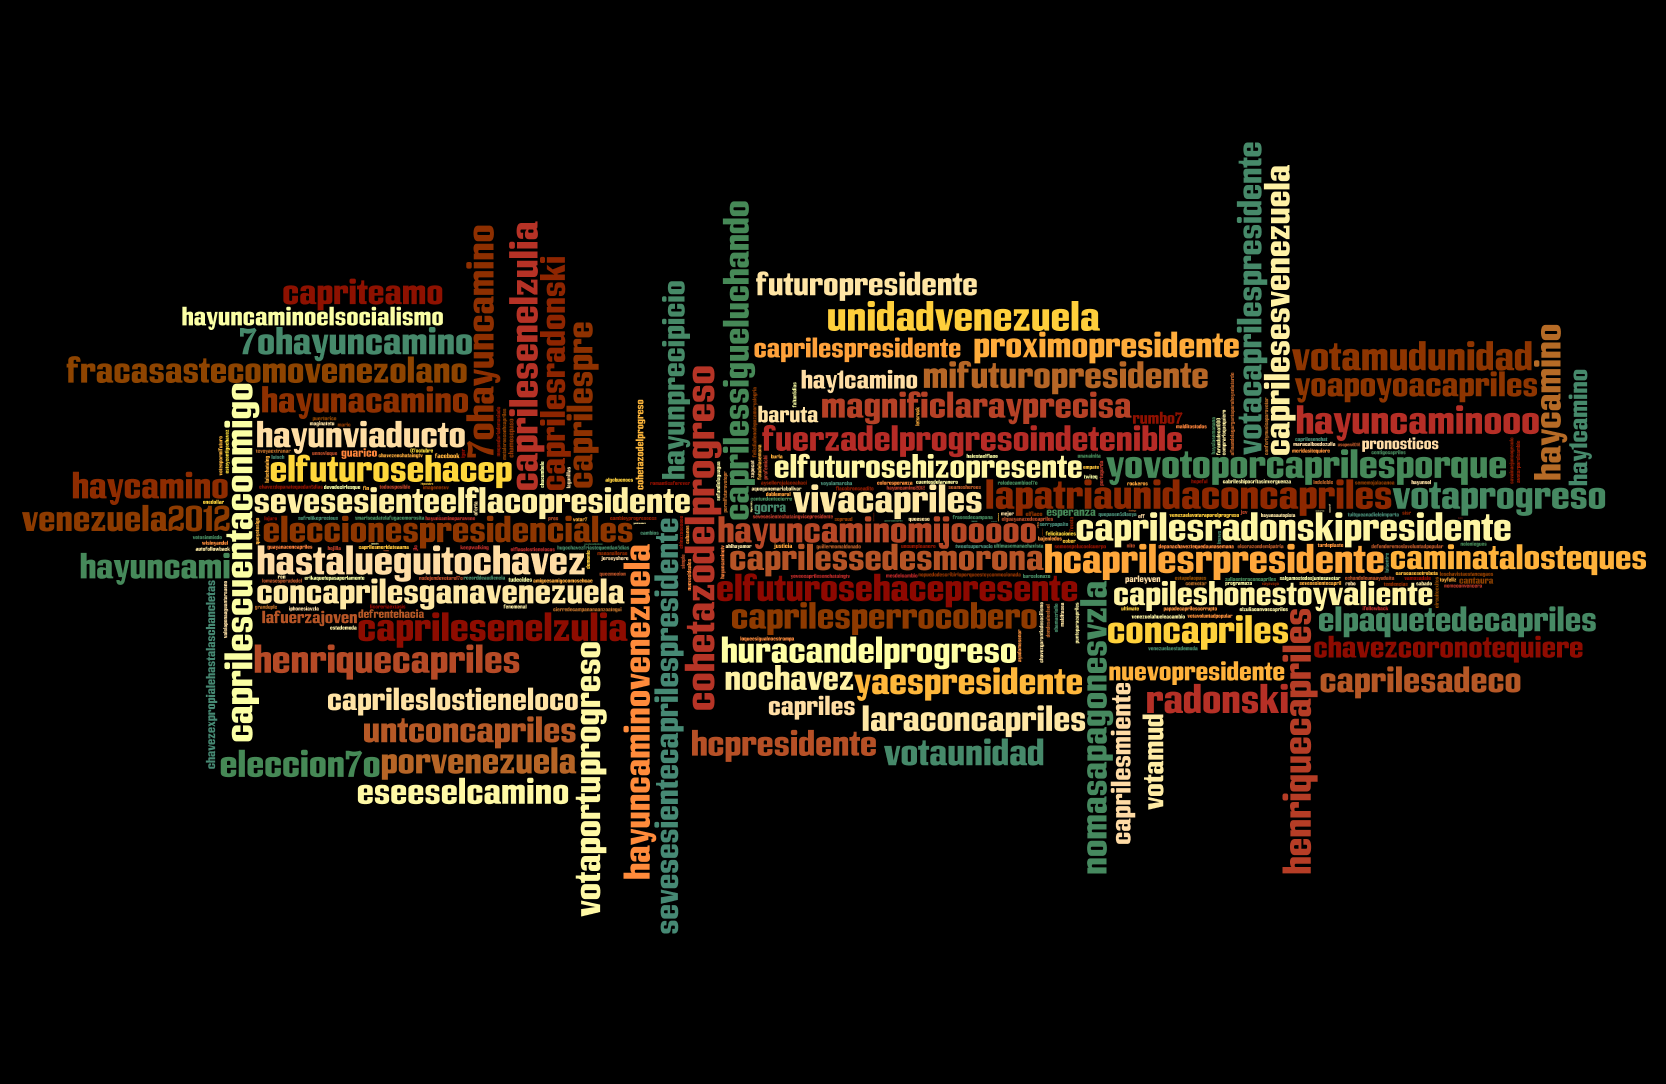
\includegraphics[width=1.0\textwidth]{/Users/aravindan/Dropbox/git/ms_thesis/documentation/my_thesis/support_files/caprilesWordCloud.png}
	\vspace{-1em}
	\caption{Word cloud for Henrique Capriles}
	\label{fig:caprilesWordCloud}
	\vspace{-1em}
\end{figure*}

Figure\ref{fig:caprilesWordCloud} shows a word cloud of hashtags which the system identified for Henrique Capriles.
It is interesting to note that hashtags like 'capriles' which was part of the initial seed vocabulary is ranked much lower than hashtags. 


